\documentclass[letterpaper]{jpconf}
\usepackage{graphicx}
\usepackage{iopams}
\usepackage[pdftex,
      colorlinks=true,
      urlcolor=blue,       % \href{...}{...} external (URL)
      filecolor=green,     % \href{...} local file
      linkcolor=blue,       % \ref{...} and \pageref{...}
      pagebackref,
      pdfpagemode=UseNone,
      bookmarksopen=true]{hyperref}


\begin{document}
% paper title
\title{Many-core applications to online track reconstruction in HEP experiments}
% Author list
\author{S.~Amerio$^1$, 
  D.~Bastieri$^1$, 
  M.~Corvo$^1$, 
  A.~Gianelle$^1$, 
  W.~Ketchum$^2$,
  T.~Liu$^3$, 
  A.~Lonardo$^4$, 
  D.~Lucchesi$^1$,
  S.~Poprocki$^5$, 
  R.~Rivera$^3$, 
  P.~Vicini$^4$
  and 
  P.~Wittich$^5$,
}
\address{$^1$ INFN and University of Padova, Italy}
\address{$^2$ Los Alamos National Laboratory, New Mexico, USA}
\address{$^3$ Fermi National Accelerator Laboratory, Illinois, USA}
\address{$^4$ INFN Roma, Italy}
\address{$^5$ Cornell University, New York, USA}

\ead{silvia.amerio@pd.infn.it}

\begin{abstract}
  %%% NSS PAPER abstract
  One of the most important issues that particle physics experiments
  at hadron colliders have to solve is real-time selection of the most
  interesting events. Typical collision frequencies do not allow all
  events to be written to tape for offline analysis, and in most
  cases, only a small fraction can be saved. The most commonly used
  strategy is based on two or three selection levels, with the low
  level ones usually exploiting dedicated hardware to decide within a
  few to ten microseconds if the event should be kept or not. This
  strict time requirement has made the usage of commercial devices
  inadequate, but recent improvements to Graphics Processing Units
  (GPUs) have substantially changed the conditions. Thanks to their
  highly parallel, multi-threaded, multicore architecture with
  remarkable computational power and high memory bandwidth, these
  commercial devices may be used in scientific applications, among
  which the event selection system (trigger) in particular may
  benefit, even at low levels. This paper describes the results of an
  R\&D project to study the performance of GPU technology for low
  latency applications, such as HEP fast tracking trigger algorithms.
  On two different setups, we measure the latency to transfer data
  to/from the GPU, exploring the timing of different I/O technologies
  on different GPU models. We then describe the implementation and the
  performance of a track fitting algorithm which mimics the CDF
  Silicon Vertex Tracker.  These studies provide performance
  benchmarks to investigate the potential and limitations of GPUs for
  future real-time applications in HEP experiments.
\end{abstract}

\section{Introduction}
%%% Verbatim from NSS paper
Real-time event reconstruction plays a fundamental role in High Energy
Physics (HEP) experiments at hadron colliders.  Reducing the rate of
data to be saved on tape from millions to hundreds of events per
second is critical. To increase the purity of the collected samples,
rate reduction has to be coupled with an initial selection of the most
interesting events.  In a typical hadron collider experiment, the
event rate has to be reduced from tens of MHz to a few kHz.  The
selection system (trigger) is usually organized in multiple levels,
each capable of performing a finer selection on more complex physics
objects describing the event. Trigger systems usually comprise a first
level based on custom hardware, followed by one or two levels usually
based on farms of general purpose processors.  The possibility of also
using commercial devices at a low trigger level is very appealing:
they are subject to continuous performance improvements driven by the
consumer market, are less expensive than dedicated hardware, and are
easier to support.  Among the commercial devices, Graphic Processing
Units (GPUs) are of particular interest for online selections given
their impressive computing power (the latest NVIDIA~\cite{bib_nvidia}
GPU architecture, Kepler, exceeds Teraflop computing power); moreover,
high-level programming architectures based on C/C++ such as
\textsc{cuda} and \textsc{opencl} make these devices more accessible
to the general user.  However, GPUs are not designed for low-latency
response, which is a critical requirement in a trigger system.

The ultimate goal of this study is to investigate the strengths and weaknesses
of GPUs when applied in a low latency environment, with particular
emphasis on the data transfer latency to/from the GPU and the
algorithm latency for processing on the GPU in a manner similar to a
typical HEP trigger application.

We showed initial studies on GPU performance in low-latency
environments ($\sim$100\,$\mu$s) in a previous paper~\cite{TIPP2011,
  NSS2012}.  In this paper we extend those studies measuring the
timing performance of different GPU cards in different data I/O
environments. The algorithm run on the GPU is a complete version of
the fast track fitting algorithm of the Silicon Vertex Tracker (SVT)
system at CDF~\cite{SVT1}. We also compare the performance of GPU
cards from different manufacturers (AMD vs NVIDIA) and different
computing environments (\textsc{cuda} and \textsc{opencl}) on the same
card. 


One of the goals of the studies is to explore using a concrete
algorithm what gains one can achieve with varying degrees of changes
to the existing algorithm. Starting with a serial algorithm
implemented on a CPU, we test an ``embarrassingly parallel'' algorithm
on the Intel MIC environment. In this case each event is handled
independently by a core on the accelerator, and the parallelization is
achieved with only minor changes to the legacy code and is only
possible in the Intel MIC environment. Next we consider an algorithm
where we unroll three internal nested loops and run these in parallel
on a GPU, using the \textsc{cuda} environment. This second approach is
programmatically more complicated and less trivial to implement. In
neither case have we re-thought the basic algorithms or the data
structures used. To achieve optimal performance, these steps would
have to be taken.  As one might expect, the improvement from the first
approach is rather modest, and the second approach shows larger
performance gains.


\section{Experimental setup and data flow}
The studies are performed on two different experimental setups,
equipped with different data transfer links and GPU cards.  In both
setups two PCs are used, one acting as a transmitter (TX) and the
other as a receiver (RX).  Data are transferred from TX to RX,
processed on the GPU, and sent back to the receiver (see
Fig.~\ref{fig_data_flow}).  The latency for a complete loop is
measured on the transmitter using the time stamp counter register.

In this setup, the transmitter can represent the detector, as
the source of the data, or an upstream trigger processor, as
the ultimate sink of the data, while the the receiver is the
trigger system: the time to transfer data to the receiver is thus a
rough estimate of the latency to transfer the data from the detector
front-end to the trigger system.
 
The input data is a set of 32-bit words, each representing a set of
hits from the detector. When the track fitting algorithm is run, the
output data is composed of 32-bit words as well, representing the
results of the fit; when the input data is not processed by the
fitting algorithm, the output data is a .... 

\section{SVT track fitting algorithm}

\section{Results}
\subsection{Data processing}
\begin{figure}[tbp]
  \centering
  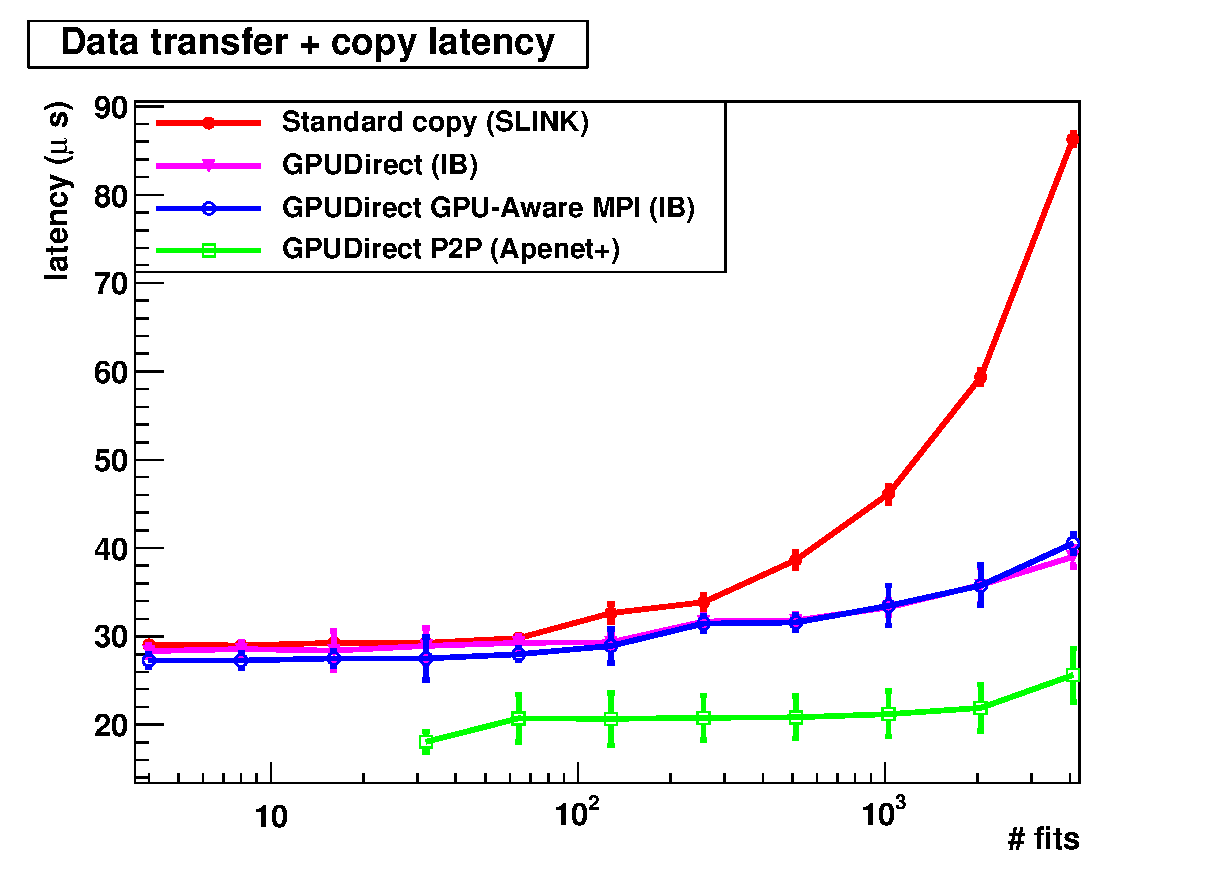
\includegraphics[width=0.9\linewidth]{../../2012/figures/DT_MC_SLINK_IB_APE_low}

  \caption{Algorithm-only comparison for timing as a function of the
    number of track fits. We compare timing on CPUs (serial), Xeon Phi
    (embarrassingly parallel), and GPUs (fully parallel.) Conclusion
    is ...}
  \label{fig:algo_only_timing}
\end{figure}
\begin{figure}[tbp]
  \centering
  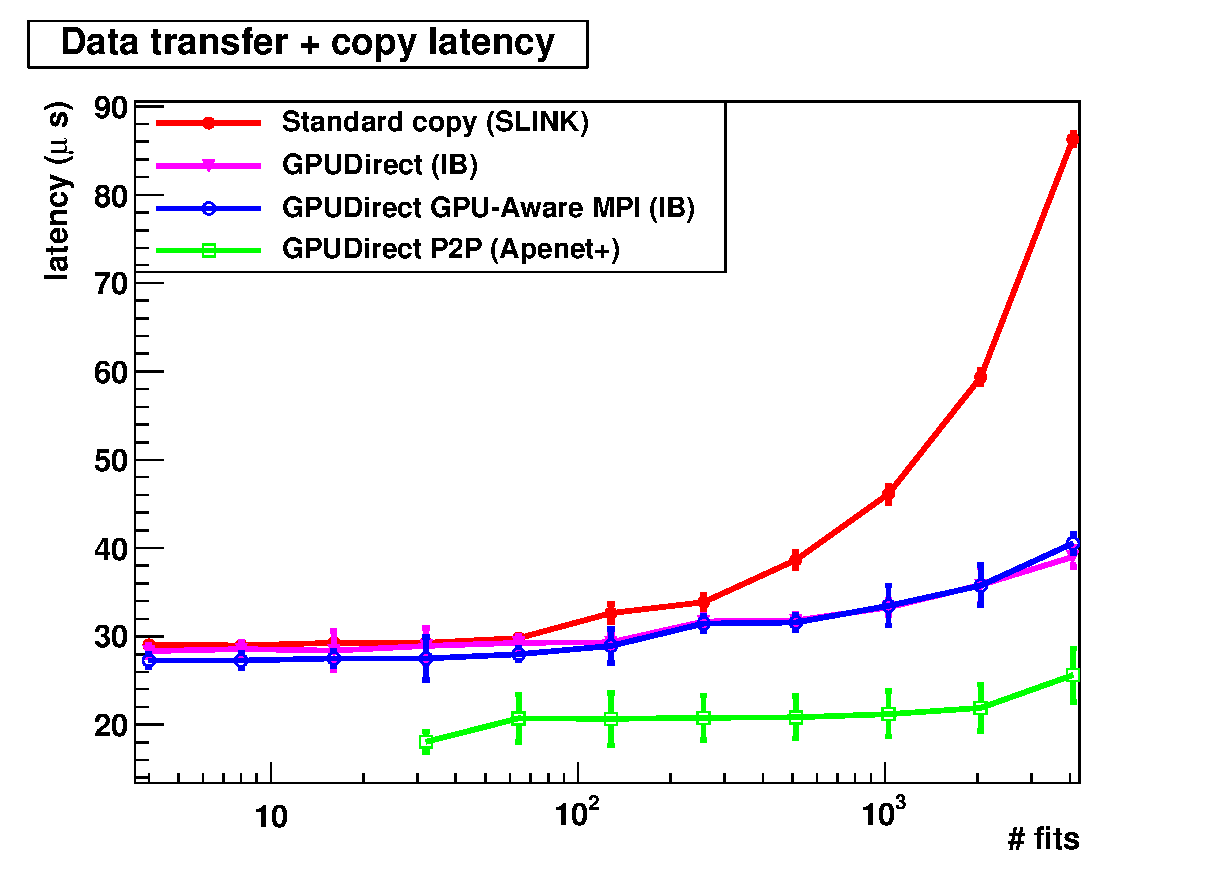
\includegraphics[width=0.9\linewidth]{../../2012/figures/DT_MC_SLINK_IB_APE_low}

  \caption{Speed-ups for algorithm-only comparison for timing as a
    function of the number of track fits. We compare timing on CPUs
    (serial), Xeon Phi (partially parallel), and GPUs (fully
    parallel.) We conclude ....}
  \label{fig:algo_only_speedup}
\end{figure}
In Fig.~\ref{fig:algo_only_timing} we compare the algorithm time as a
function of the number of fits performed, for the serial,
embarrassingly parallel and parallel algorithms. We see that the
embarrassingly parallel algorithm gives a modest increase with respect
to the serial (CPU) algorithm. Switching to a fully parallel algorithm
affords a much more significant speed
improvement. Fig.~\ref{fig:algo_only_speedup} shows the speed-up for
each... do we want to show this. Not a lot of new information.

\subsection{Breakdown of computing time}
\begin{figure}[tbp]
  \centering
  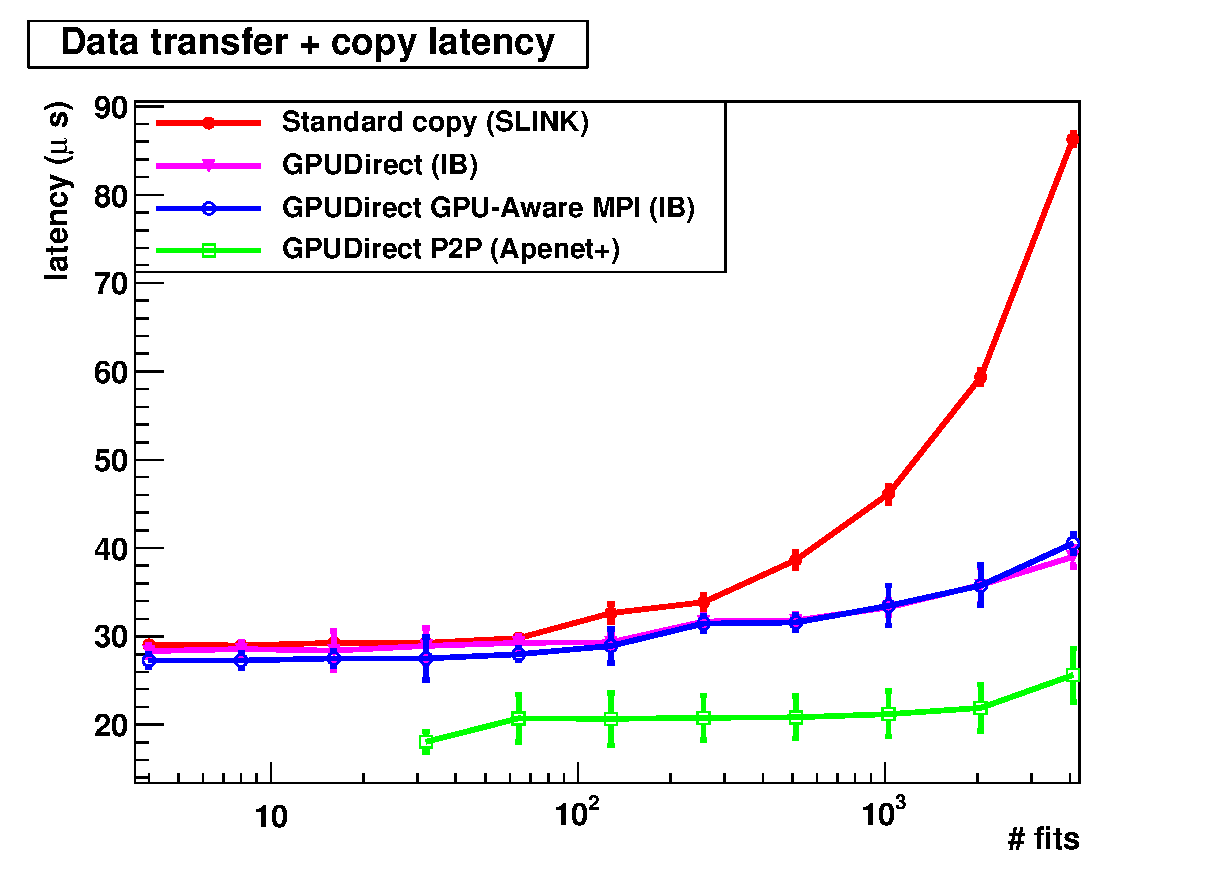
\includegraphics[width=0.9\linewidth]{../../2012/figures/DT_MC_SLINK_IB_APE_low}
  \caption{breakdown of computing time}
  \label{fig:breakdown}
\end{figure}
In Fig.~\ref{fig:breakdown} we show the fractional time spent in
various parts of the algorithm for the serial algorithm (on a CPU),
the embarrassingly parallel algorithm (on Intel MIC) and the parallel
algorithm (on NVidia GPUs), as a function of the number of
fits. Interesting features are ...

%% gives unnumbered ack in CHEP style
\ack
The authors would like to thank the Fermilab staff and the FTK group at the 
University of Chicago for their support. This work was supported by the
U.S. Department of Energy, the U.S. National Science Foundation and the Italian
Istituto Nazionale di Fisica Nucleare. 


%% CHEP2013 recommended style for bibliography
\bibliographystyle{iopart-num}

\bibliography{gpu}

 
\end{document}


